\chapter{绪论}
\section{引言}
白癜风是一种常见的皮肤色素脱失病,影响全世界0.5\%到1\%的人群,该病的主要特征是在体表形成大小无规则的白斑皮损,是一种严重影响外貌美观的疾病, 白斑面积是临床治疗效果的重要评价指标,白癜风在评估方法上缺乏共识,这使得分析或比较不同研究的结果变得困难。而测量白斑面积的基础则是准确将白斑区域分割出来。

传统的白斑面积测量方法有目测估算法、点估算法、宫格法等\cite{林瑶2002医学图像分割方法综述}。但是由于其主观性强,缺乏客观的衡量标准,逐渐被基于图像分析的测量方法所取代。例如,目测估算法通过医生的主观判断,将病人分为几个患病等级,从而实施治疗方案;点估算法与宫格法是将透明度的塑料薄片贴于患处表面,通过人工拓取患病区域进而测量患病面积。这些传统方法缺乏客观评估且操作繁琐。随着图像处理技术的发展,基于图像分析的测量方法可以做到非接触式测量,客观准确,但由于图片拍摄环境、拍摄器材、患者皮肤自身的色度等诸多因素的限制,做到将白癜风区域高效,准确的分割出来仍具有一定难度。如基于混合颜色空间的K均值聚类方法\cite{2006数字图像处理}采用将输入的RGB图像转转换到CIELAB、HSV、YCbCr空间中进行K均值聚类分割,但该方法需要同时在三个空间下进行聚类,计算量大,难以对分辨率高的图像进行有效的处理,且以像素点为最小单位进行分割;使用Photoshop或者其他图像处理工具对白癜风区域进行手动分割,标记边缘的方法,效果虽精确但操作繁琐;基于snake模型对白癜风皮损边缘进行提取的方法,要求先给定目标区域的初始轮廓,且算法对噪声较为敏感,且设备要求高。使用YCbCr颜色空间与Fuzzy C-Means (FCM) 聚类相结合的方法,虽然达到了不错的分割效果,但无法适应图片对比度较小的情况。

因此,根据现存方法的一些缺点,如计算量大,操作繁琐,对拍摄器材要求高,只适用于强对比度的图片等,本文提出了一个高效、简单、鲁棒性强的白癜风区域分割方法,这将有助于推进白癜风的评价体系的客观化,标准化进程。且在一定的场景下,改方法同样可应用于其他病种皮损区域的分割。

\section{研究现状}
\subsection{白癜风评价体系}
白癜风在评估方法上缺乏共识,这使得分析或比较不同研究的结果变得困难。早期,白癜风欧洲任务小组(VETF)\cite{taieb2007definition}和白癜风面积评分指数(VASI)\cite{Iltefat2004Parametric}提出了更准确的疾病严重程度指数和治疗评估标准。

VETF 是一个综合的评分系统,其从白癜风的范围、阶段及进展三个方面综合评价。白癜风的范围采用传统的“九分法”测量,以患者手掌为体表面积1\% 估算,将身体分为四个部分:头和颈部( 0 ~ 9\%) 、躯干( 0 ~ 36\%) 、上肢( 0 ~ 18\%) 、下肢( 0 ~ 36\%) 。手和足在评价白癜风范围时分别纳入到上肢和下肢中评价,但在评价白癜风的阶段和进展时,则作为独立部分单独评价。白癜风的阶段则参考伍德灯下检查的结果进行评估,分为四个等级。零等级:正常肤色( 区域内无脱色) ;一等级:不完全正常肤色( 包括斑点脱色,这一阶段的少许白色毛发不影响阶段评级) ; 二等级: 完全脱色( 这一阶段的少许白色毛发不影响阶段评级) ; 三等级: 完全脱色,并伴随部分毛发变白( < 30\%) ; 四等级: 完全脱色,并伴随毛发完全变白。% cite 白癜风评估方法VETFa 和VASI 的介绍 王禹
白癜风的进展则是通过比较自然光下与伍德灯下皮损的边界。分为三个等级:边界相似、进展期白癜风( 持续的脱色) 、恢复期白癜风( 持续的复色) 。

VASI的目的是使医生能测量患者不同时间复色、脱色情况及治疗后的疗效。以患者手掌为体表面积1\% 估算,患者身体被分为5个独立的部分: 手,上肢,躯干,下肢和足,来估算身体每个部位白斑的面积。在每一次统计的过程中,每一皮损按照脱色程度分为7 个等级:0\%,10\%,25\%,50\%,75\%,90\% 或100\%, 如图\ref{fig:chap1_VASI}所示。100\% 表示完全白化,0\%表示正常无脱色。将每一部分内的皮损面积(以手掌单位) 乘以脱色程度得到每一部分的得分,将每一部分得分相加构成了整个身体的VASI 得分( 0 ~ 100 分).

近些年,还有一些其他的方法在以上两种经典的方法的基础上被提出,他们基于精心设计的病情问诊流程,包括从患者和专家两方面来评估病变的面积和严重程度,从而实现了更好的评估者内部可靠性\cite{feily2014vitiligo,van2016development}。
\begin{figure}[htbp]
\begin{center}
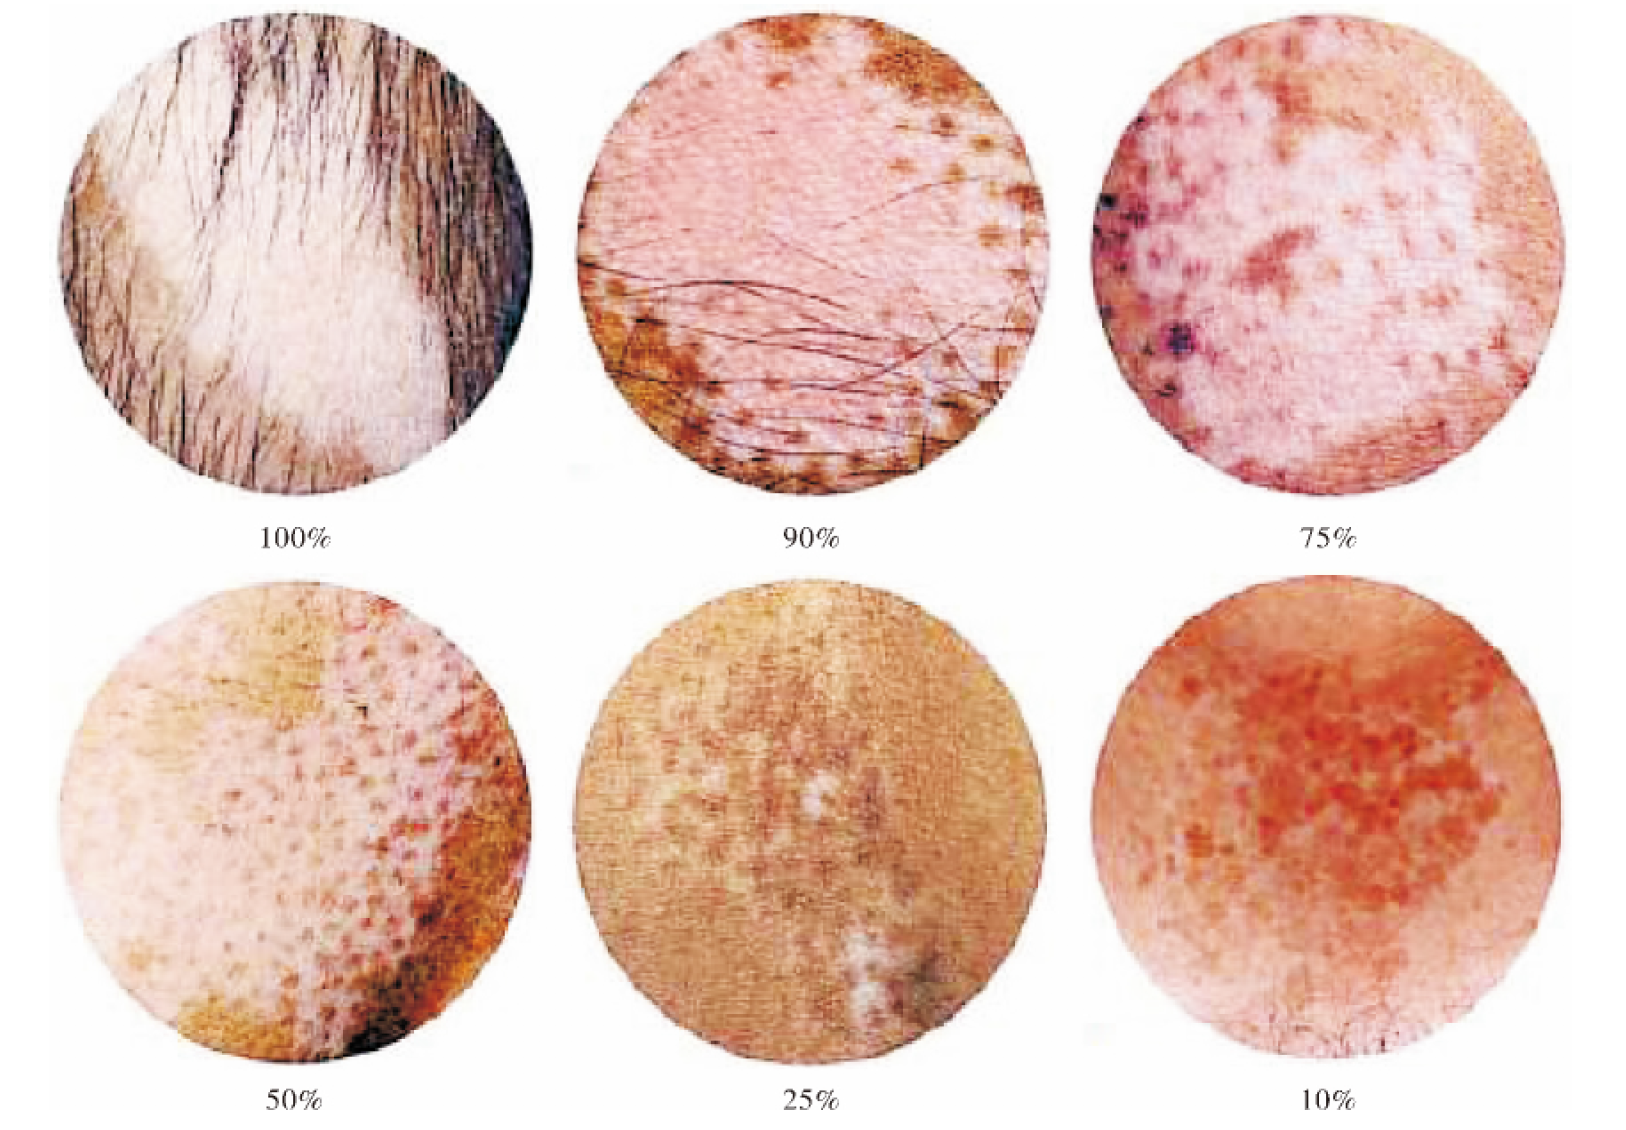
\includegraphics[width=0.7\linewidth]{chap1_VASI.png}
\end{center}
\caption{VASI指标白癜风脱色程度参考}
\label{fig:chap1_VASI}
\end{figure}
直到最近,研究人员才开始尝试以较少的人为干预来探索新的基于面积测量的评估,例如点计数方法,例如~\cite{aydin2007practical},planimetry~ \cite {aydin2007practical}和数字化方法\cite {marrakchi2008objective, verma2015evaluation}。但是,昂贵的设备和软件以及这些方法中的低效操作使其不太实用。例如,将透明薄片放置在白癜风病变上并用普通笔勾画边界,然后通过计算网格上的点或用CAD软件计算来测量该区域。因此,在产生大量图像的真实临床场景下应用这些方法是不实际的。

综上,本文发现目前所应用的白癜风评价体系大都是半客观的、基于专家或者病人本身的估算而评价的,难以做到客观评价。若要对其进行客观的评价,则需要精确的测量出白癜风边界的面积,而此前提便是对白癜风区域进行精确的分割。

\subsection{色素性皮肤病分割}
白癜风作为非常具有代表性的色素性皮肤病,其很多分割的方法都借鉴于色素性皮肤病的分割方法。

色素性皮肤病变图像分割的主流是基于边缘的方法、基于阈值的方法、基于区域的方法和深度学习方法。许多基于边缘的方法已应用于皮肤病变图像\cite {barcelos2009automatic,de2011skan}。然而,产生的边缘是不连续的并且对噪声敏感。阈值处理方法已被广泛应用于皮肤病变分割任务中\cite{norton2012three,abbas2013perceptually,cavalcanti2013coarse},此方法的原理较为直观,而且实现起来也很高效。但是对于对比度低的白癜风图像,该方法很难适用,因为难以选取准确的阈值边界。基于区域的增长、分裂和合并算法也已经被用于皮损区域的分割\cite{castillejos2012wavelet, de2011skan, wong2011automatic}。该方法的核心是选取一些种子点,然后采用一定的度量手段来对其周边的像素或者区域进行差异性度量,然后再采取合并或者分裂的操作。基于区域的方法已经显示出对图像噪声、不同的光照条件和低对比度的鲁棒性。
%其优点是实现相对简单,对于物体灰度值或其他特征值相差很大时,能很有效的对图像进行分割。其缺点是不适用于特征值相差不大的图像,对于图像中不存在明显的灰度差异或各物体的灰度值范围有较大重叠的图像分割问题难以得到准确的结果,这些方法可能产生比实际更小的片段并且导致非常不规则的病变边缘。增长区域算法、分裂和合并操作是典型的基于区域的技术,其特点是将分割过程分解为多个步骤,其中后续步骤要根据前面步骤的结果进行判断而确定。区域生长的基本思想是将具有相似性质的像素集合起来构成区域,该方法需要先选取一个种子点,然后依次将种子像素周围的相似像素合并到种子像素所在的区域中。这类方法已被用于分割皮肤病变\cite{castillejos2012wavelet, de2011skan, wong2011automatic}。


深度学习\cite{2010模式识别, 2016机器学习}已被应用于分割任务。例如人工神经网络\cite {schaefer2011colour, rajab2004application,2010模式识别},将图像分割问题转化为分类问题或者求解能量函数最小化等问题。其基本思想是用大规模数据集对网路进行训练,再用训练好的人工神经网络去分割。

近期,在人工神经网络的基础上有学者提出了完全卷积神经网络\cite{ 2018深度特征融合的图像语义分割, long2015fully, noh2015learning, ronneberger2015u}。完全卷积神经网络对图像进行像素级的分类,从而解决了语义级别的图像分割问题。与经典的卷积神经网络不同,完全卷积神经网络可以接受任意尺寸的输入图像,采用反卷积层对最后一个卷基层的特征图进行上采样,使它恢复到输入图像相同的尺寸,从而可以对每一个像素都产生一个预测,同时保留了原始输入图像中的空间信息。其中这种模型具有更快的速度和精确度。但其也存在相应的问题,例如数据集的获取需要大量的人工操作。从监督的角度上来看,不论是完全卷积神经网络还是人工神经网络,他们都需要大量的数据和监督信息,而在医疗图像领域,监督信息的获取又十分的困难。因此本文的贡献之一是提出了一种弱监督的分割方法,只需要利用图像的类别标签,即可完成对皮损区域的分割。

\subsection{白癜风图像的分析与分割}
针对白癜风的特点,一些学者也进行了一些研究。基于18名患者的41个白癜风区域的数字图像,Nugroho 等人 \cite {nugroho2013computerised}应用主成分分析(PCA),然后进行独立成分分析(ICA),分别将白癜风图像分为黑色素和血红蛋白成分两个成分。研究人员报告说,皮肤颜色是由于皮肤载色体组成,即黑色素和血红蛋白的组合。然而,在数字彩色成像中,通过组合三个光谱带产生颜色:红色,绿色和蓝色(RGB)。于是,在该算法中,主成分分析(PCA)用于将尺寸从三个(RGB)颜色通道减小到两个主要成分。接下来,ICA用于对齐两个主要成分轴以代表黑色素和血红蛋白,参见图\ref{fig:PCA}。然后白癜风皮肤区域被确定为缺乏黑色素的皮肤区域。在该方法中,首先确定一组种子点,然后使用区域增长算法,即从这些种子中,通过向每个种子附加具有与种子相似的属性的相邻像素来实现区域的增长。

\begin{figure}[htbp]
\begin{center}
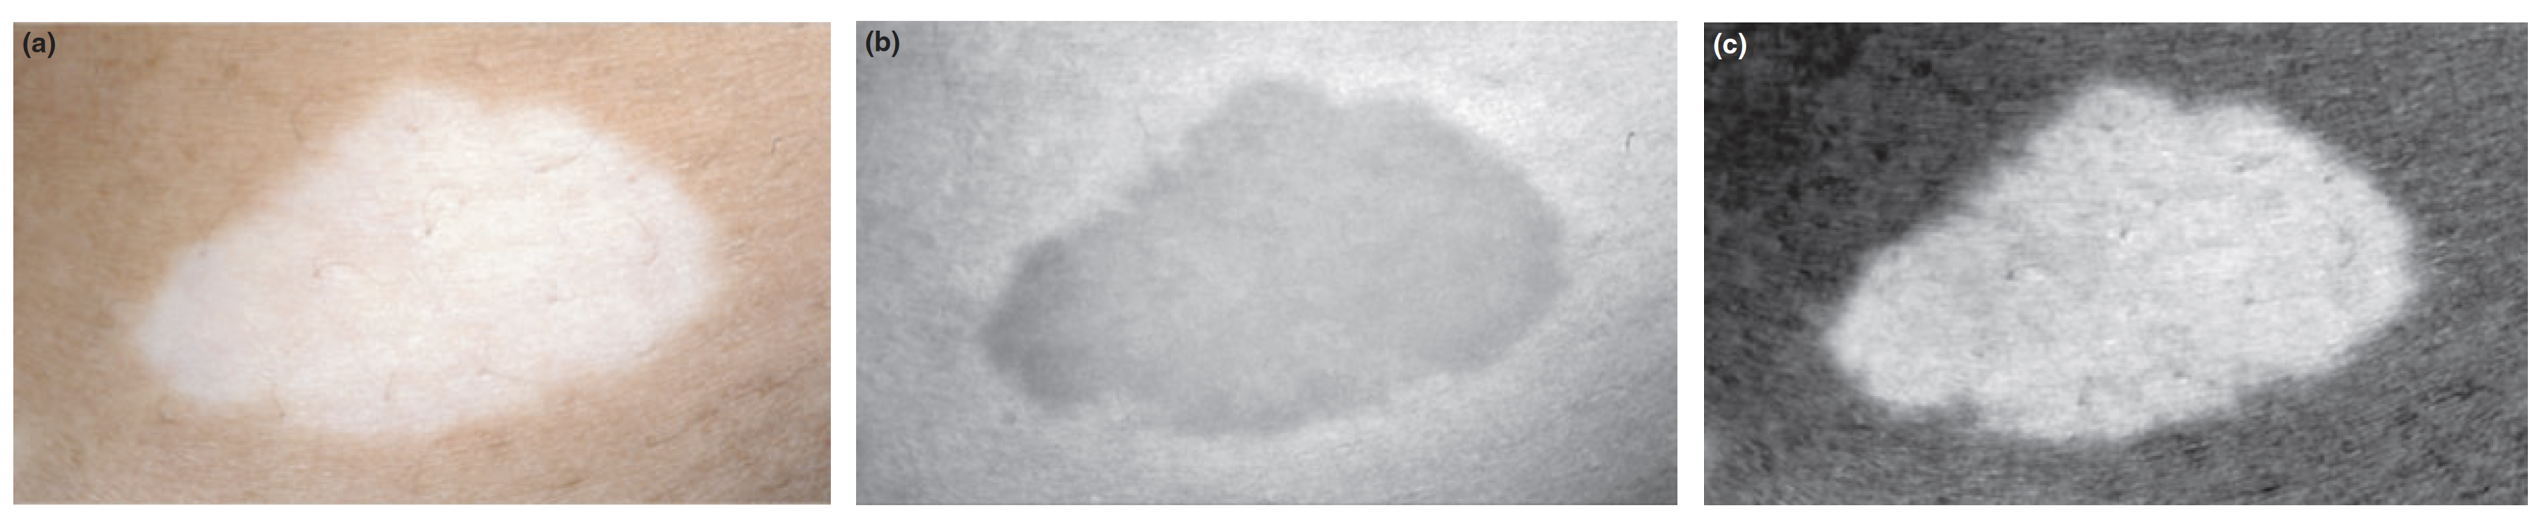
\includegraphics[width=\linewidth]{PCA.png}
\end{center}
\caption{PCA-ICA的例子。 (a)原始皮肤图像 (b)皮肤区域由血红蛋白引起的颜色(血红蛋白图像)(c)皮肤区域图像由黑色素引起的颜色(黑色素图像)}
\label{fig:PCA}
\end{figure}

但由于该方法所涉及的皮损区域较为简单,其算法在复杂场景不具备鲁棒性。但是其从医学方面分析白癜风形成的原因,这一角度为后面的研究提供了宝贵的经验。

Nurhudatiana 等人 ~ \cite {nurhudatiana2015computer}分别在YCbCr和RGB颜色空间的Cr和Blue通道中进行模糊C均值聚类,以分离图像中的背景、皮肤、皮损区域。 使用YCbCr颜色空间是因为YCbCr颜色空间中的CbCr二维平面的大Cr值的坐标非常好地定位了肤色。使用FCM算法是因为皮肤的像素倾向于在图像中形成均匀的簇,因此可以将皮肤分割作为聚类问题来处理。

\begin{figure}[htbp]
\begin{center}
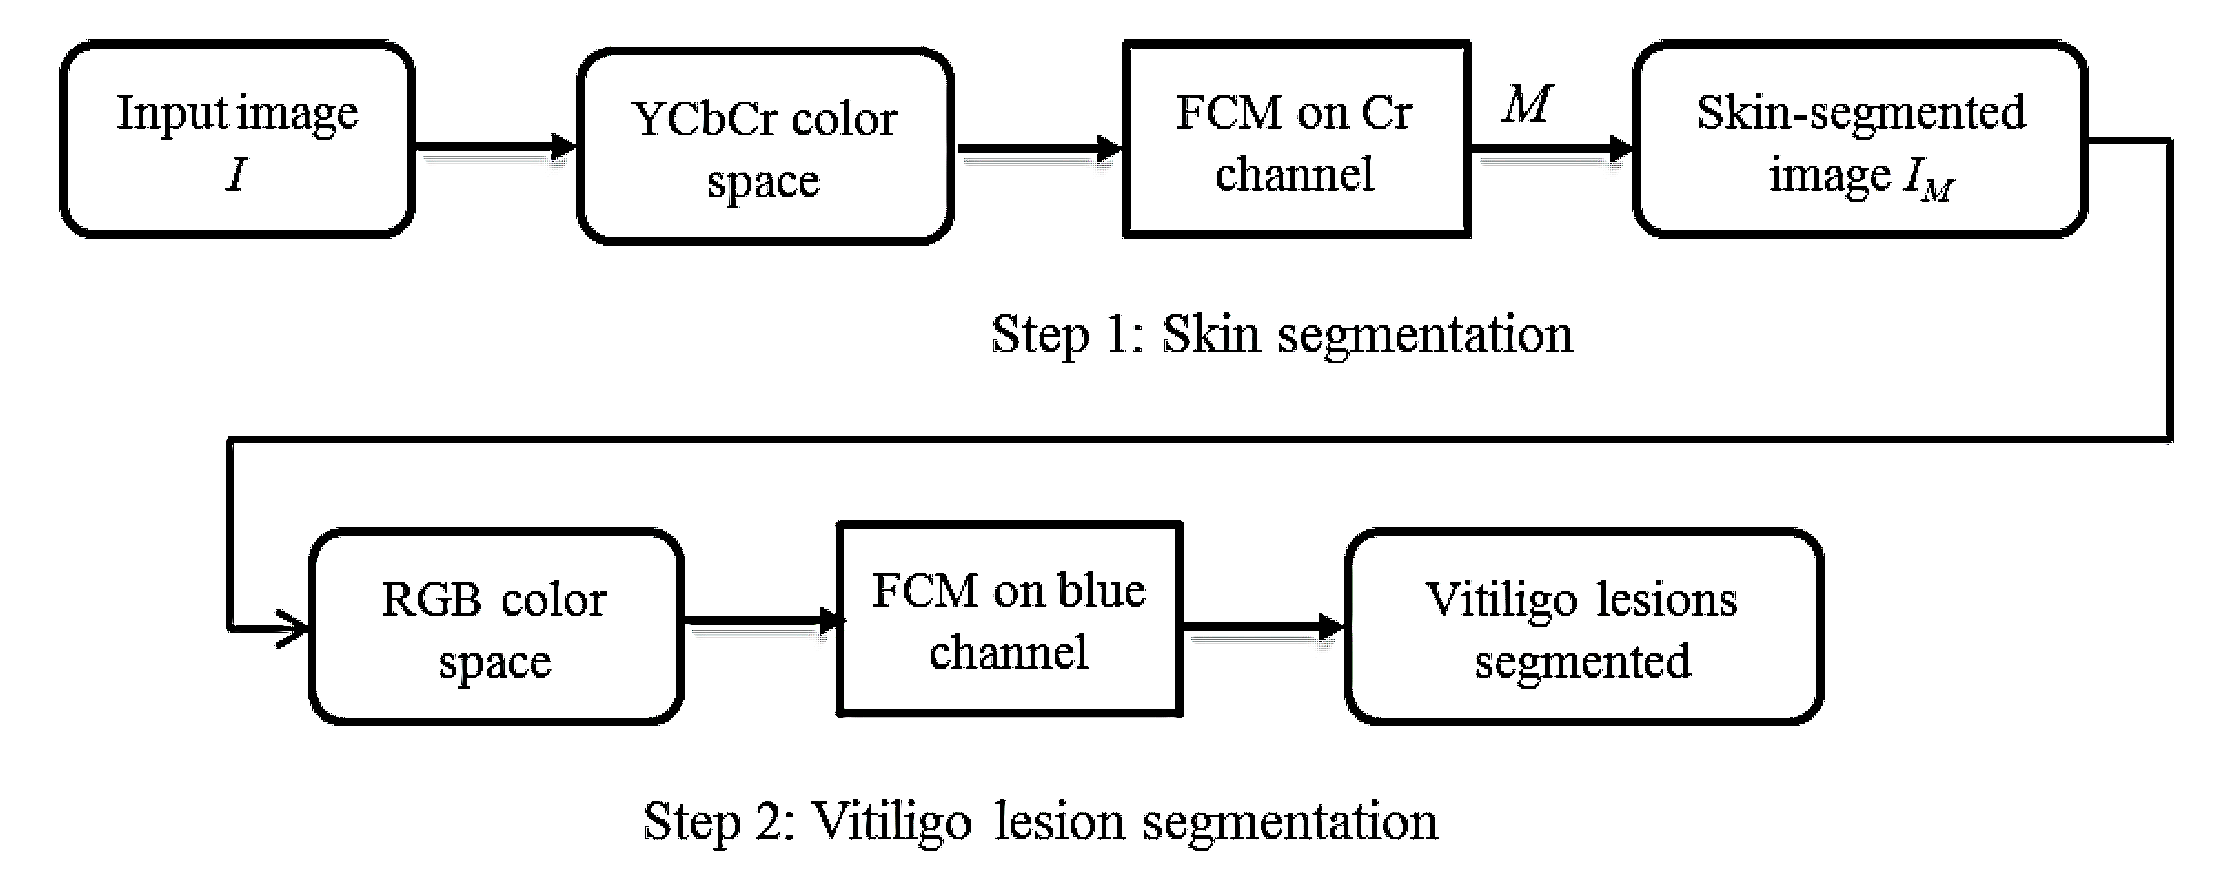
\includegraphics[width=0.9\linewidth]{FCM1.png}
\end{center}
\caption{结合YCbCr与FCM 方法流程图 \cite {nurhudatiana2015computer}}
\label{fig:FCM1}
\end{figure}

其所提出的算法如图\ref{fig:FCM1}所示。该算法由两个步骤组成。第一步是皮肤分割步骤,其用作预处理以定位图像中的皮肤区域,第二步是白癜风病变分割步骤。皮肤分割步骤的工作原理如下。给定输入RGB图像,首先将图像变换为YCbCr颜色空间以进行皮肤分割。然后使用均值滤波器提取和平滑Cr通道。然后使用模糊C均值(FCM)聚类算法将平滑后的通道分割成两个不同的聚类。由于皮肤趋向于在Cr通道中具有高强度值,因此以在通道Cr中10和90百分位的强度值的位置初始化聚类中心,其中第一簇表示背景,第二簇表示皮肤。该过程产生皮肤掩模M(参见图\ref{fig:FCM2})。

\begin{figure}[htbp]
\begin{center}
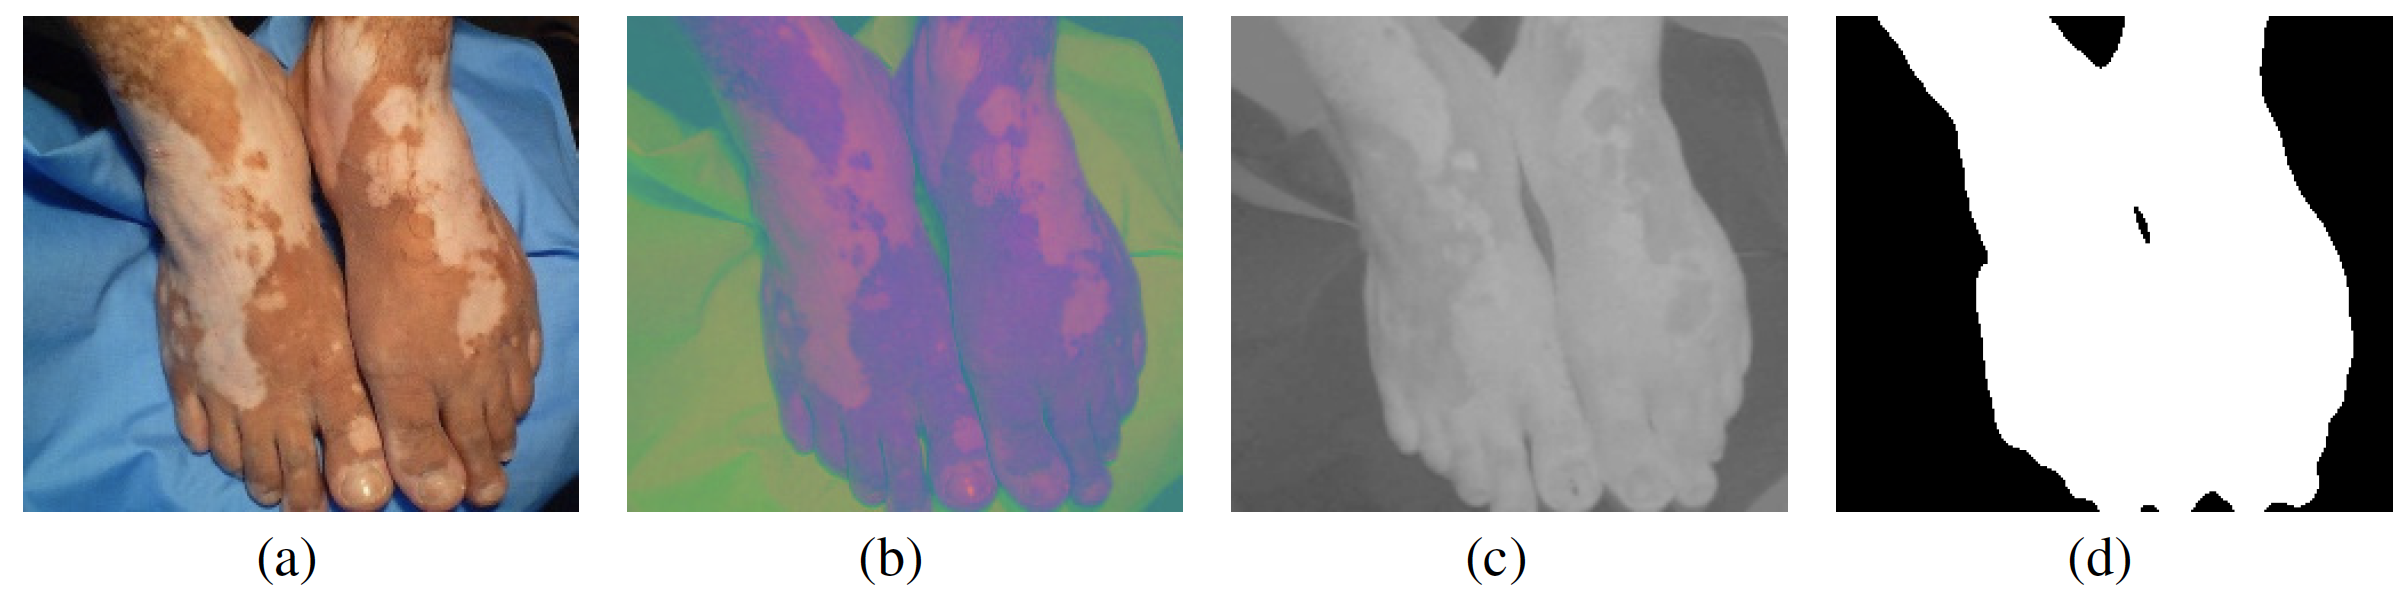
\includegraphics[width=0.9\linewidth]{FCM2.png}
\end{center}
\caption{皮肤分割过程 \cite {nurhudatiana2015computer}。(a) 输入RGB图像,(b) YCbCr颜色空间中的输入图像,(c) 从(b)中提取的Cr通道,以及(d)皮肤掩模$M$}
\label{fig:FCM2}
\end{figure}

然后使用形态学操作器平滑皮肤掩模$M$,该操作移除尺寸小于图像像素分辨率的10%的所有连通分量。将蒙版$M$应用于输入图像以获得皮肤分割图像$I_M$,其中属于第一聚类(背景)的像素的值被设置为零,并且属于第二聚类(皮肤)的像素的值被保留。经过皮肤分割后,还需要再进行白癜风皮损区域分割。在该步骤中,使用不同的颜色通道,尤其是RGB颜色空间的蓝色通道。蓝色通道波长接近紫外波长,而红色和绿色通道的波长穿透皮肤的较深层。因此,与红色通道和绿色通道波长相比,皮肤对蓝色通道波长更敏感。图\ref{fig:FCM3}比较了红色,绿色和蓝色通道中白癜风皮肤的外观。

\begin{figure}[htbp]
\begin{center}
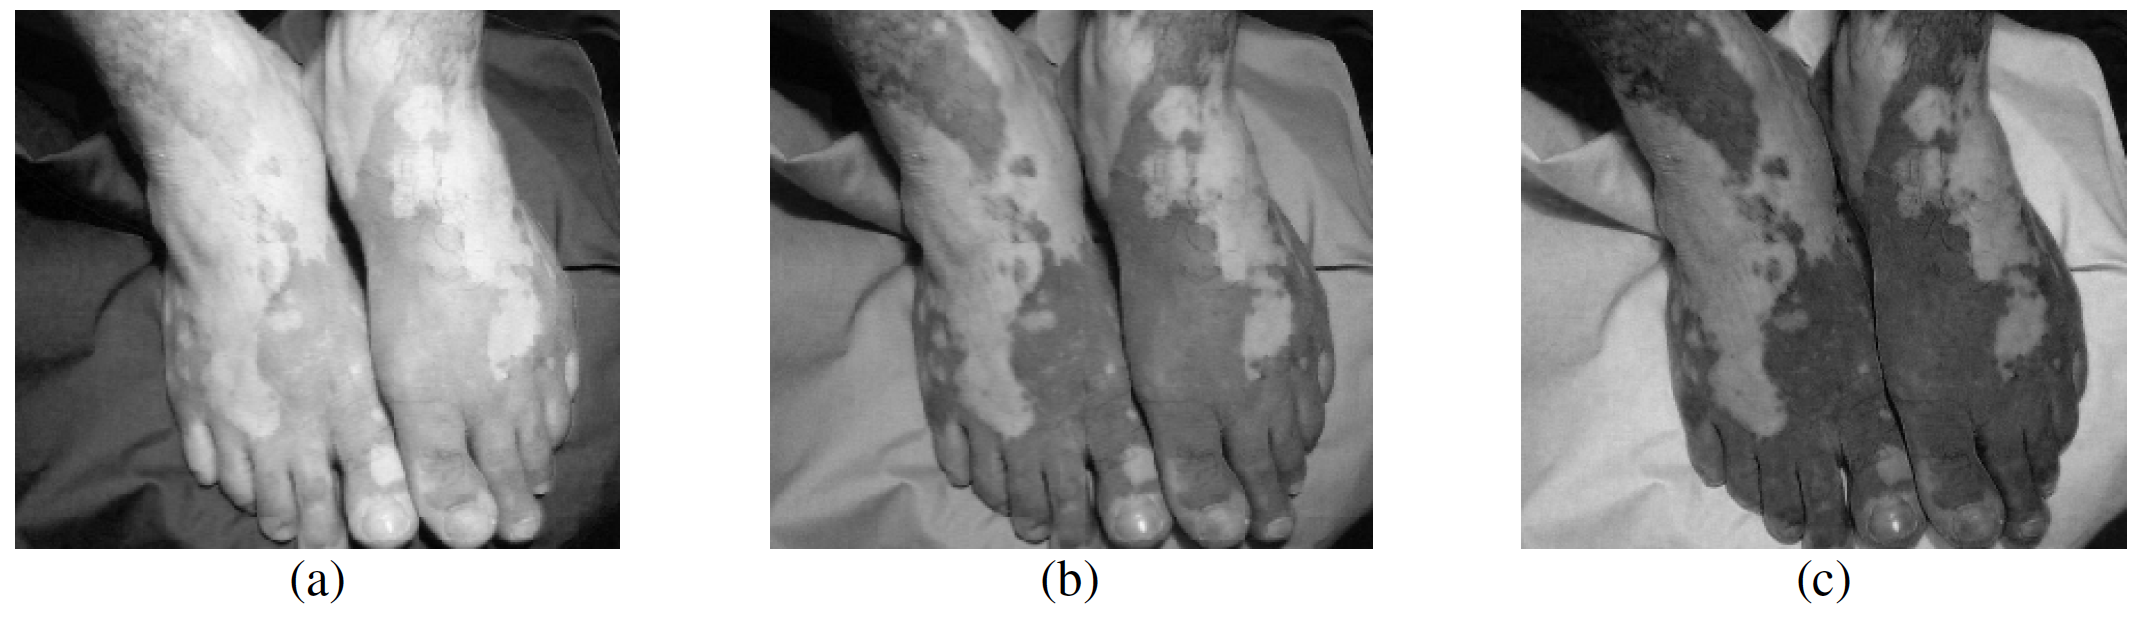
\includegraphics[width=0.9\linewidth]{FCM3.png}
\end{center}
\caption{白癜风皮观在(a)红色通道,(b)绿色通道和(c)蓝色通道中的比较 \cite {nurhudatiana2015computer}}
\label{fig:FCM3}
\end{figure}

可以观察到,与其他通道相比,正常皮肤和脱色皮肤之间的对比度差异在蓝色通道中最高(如图\ref{fig:FCM3}所示).然后同样将FCM聚类操作应用于分割好的皮肤图像。然后基于质心值进一步对得到的聚类进行分类。质心几乎等于零的簇表示黑色背景,因此在皮肤图中用黑色标记,而剩余的两个具有非零质心的簇表示皮肤。具有较低质心值的簇表示着色皮肤的像素,因此在皮肤图中用灰色标记,而具有较高质心值的簇表示脱色皮肤的像素,因此在皮肤图中用白色标记。

该方法利用白癜风对紫外线敏感的特征,对白癜风皮损区域达到了较好的分割效果。但是由于照片的拍摄环境不同,患者的皮肤肤色不同,会使得该先验知识在一定环境下失效。且方法中许多阈值需要人为手工确定,难以适应大量图像的自动化处理。

近些年来,还有一些基于超像素的分割方法,通过使用不同的视觉特征或超像素尺度聚合超像素。Mithun 等人~ \cite {das2015kl}提出了一种基于对称Kullback-Leibler散度的凝聚聚类方法,用于分割白癜风图像中的多种脱色水平,如图\ref{fig:KL1}。

\begin{figure}[htbp]
\begin{center}
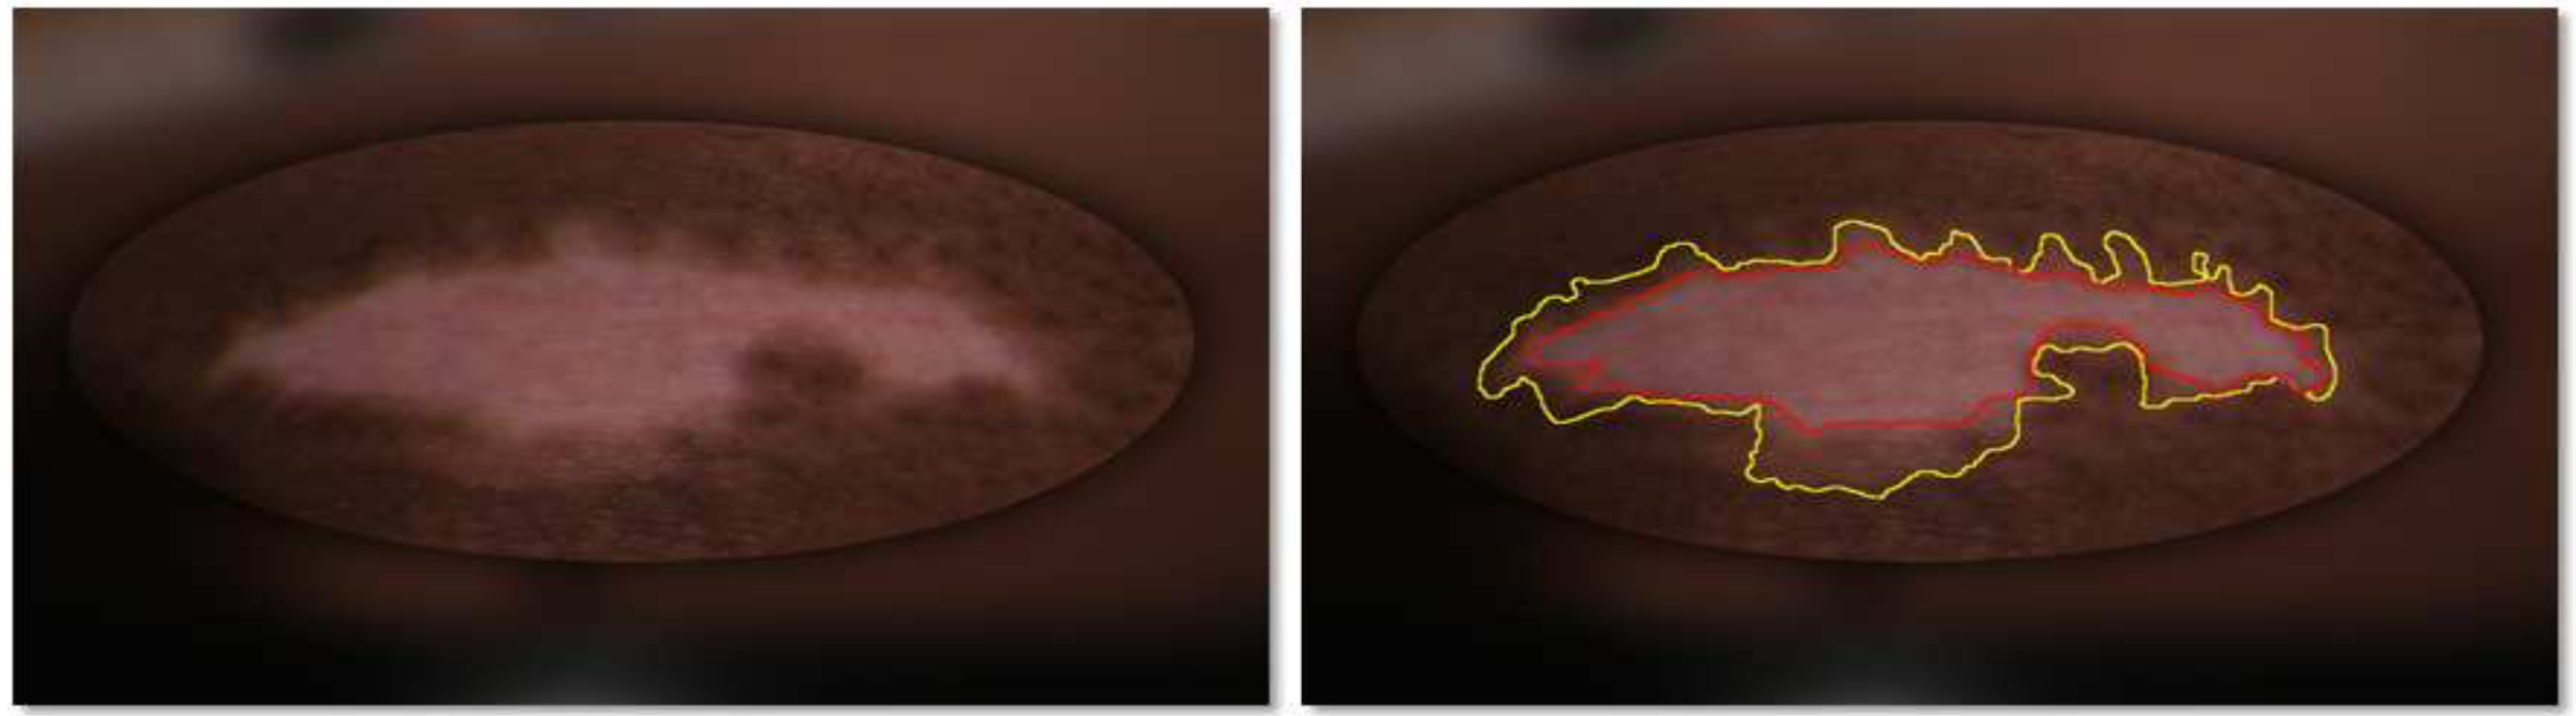
\includegraphics[width=0.9\linewidth]{intro.png}
\end{center}
\caption{⽩癜风分割及其专家标注\cite {das2015kl}。红⾊边界标志着完全脱⾊的⽪肤。黄⾊边界表⽰部分脱⾊的⽪肤。}
\label{fig:KL1}
\end{figure}

他们首先提出了两个正态分布的簇之间的对称Kullback-Leibler(KL)散度(等式\ref{eq:KL2}),作为距离度量。
\begin{IEEEeqnarray}{rCl}
\label{eq:KL1}
KL_{C_i,C_j}&=&\frac{1}{2}(tr({\Sigma_j^{-1}\Sigma_j^{-1}})+(\mu_j-\mu_i)^T\Sigma_j^{-1} \nonumber \\
&& (\mu_j-\mu_i)-d-\ln{\frac{|\Sigma_i|}{\Sigma_j}})
\end{IEEEeqnarray}
\begin{equation}
\label{eq:KL2}
D_{SKL}(C_i,C_j)=KL_{C_i,C_j}+KL_{C_j,C_i}
\end{equation}
其中$C_i$和$C_j$表示簇,$(\mu,\Sigma)$表示特征均值和协方差,d是特征维度。 对数项和逆协方差项在公式中是明显的瓶颈,这使得研究人员不使用基于KL散度的成本函数。 在协方差不为奇异的情景中,KL散度被证明是非常有用的散度度量。 对于基于区域的皮肤图像,特征上的协方差很少达到零。 此外,他们在协方差矩阵中加一个小分量\cite{Gupta2011Non},以保证迹的有界性。 

在这种对称的KL散度基础上,他们使用自下而上的分层凝聚聚类算法进行白癜风图像的分割。使用超像素作为图像基元图像特征,以降低后续图像处理任务的复杂性。他们观察到由于白癜风是一种表皮疾病,患者部分或完全丧失皮肤着色,这导致患病斑块的更高反射。于是将白癜风斑块分解成反照率区域和阴影区域图像。他们根据不同的脱色阶段,引入反照率和阴影图像作为白癜风区域分割的特征。其参照了 Zhu和Yuille\cite{zhu1996region}在关于区域竞争的论文中提出的用反照率图像进行皮肤图像分割的方法。

每个像素的特征向量具有十个维度,是由以下加权的矩阵堆叠而成。 记LAB为CIELAB彩色图像(3通道),RGB为彩色图像(3通道),A为反照率图像(3通道),S为阴影图像(3通道),$L=\Sigma_cI^c/\Sigma_cI$( 单通道)为图像的亮度。那么特征图像$I_f$就可以表示为:
\begin{equation}
\label{eq:2}
I_f
\begin{bmatrix}
LAB*(1+\gamma S))\\ 
\alpha RGB*(1+\gamma S))\\ 
\beta A*(1+\gamma S))\\ 
\kappa L
\end{bmatrix}
\end{equation}
其中$\alpha,\beta,\gamma$ 和 $\kappa$是自由参数,来加权不同的图像,$*$表示将每个通道相乘。 其算法思路见表\ref{tab:addlabel}
% Table generated by Excel2LaTeX from sheet 'Sheet1'
\begin{table}[htbp]
  \centering
   \caption{基于KL散度的图像分割层次聚类算法}
    \begin{tabular}{l}
    \toprule
    \textbf{算法1} 基于KL散度的图像分割层次聚类算法 \\
    \midrule
    \multicolumn{1}{p{28.2em}}{需要RGB彩色图像,最终聚类数量$c_F$生成反照率(A)和阴影(S)图像生成超像素} \\
    \textbf{重复} \\
    \hspace{1em}为集群生成邻接矩阵 \\
    \hspace{1em}计算特征空间中相邻超像素的成对亲和度 \\
     \hspace{1em}合并具有最低亲和力的两个群集并更新群集统计信息 \\
    \textbf{直到} 簇数等于 $c_F$ \\
    返回最终簇 \\
    \bottomrule
    \end{tabular}%
   
  \label{tab:addlabel}%
\end{table}%

然后设计了一种自上而下的聚类技术,将最后几个聚类合并到具有生理意义的标签上。但是对于不同图像的聚类停止规则难以统一。为了解决这个问题,他们为所有方法提出了一个停止准则,即$c_F = 15$,其中$c_F$在算法1中定义。

虽然该方法可以分割出不同脱色程度的白癜风区域。但是,对于一些较复杂在的情况,该方法仍然难以胜任,而且由于统一了自下而上聚类算法的停止准则,所以对不同图片的处理效果也良莠不齐。

综上,本文的方法相比于目前的皮损区域分割或者白癜风区域分割的方法,优势在于:
\begin{enumerate}
\item 无需任何人为干预的自动分割;
\item 基于弱监督的分割,无需做像素级别的人工标注。
\item 在不同环境下,分割效果具有很强的鲁棒性。
\end{enumerate}

\section{面临挑战}
在具体的临床应用中,我们往往会遇到很多实际的问题,而目前很多的研究方法均是在一些公开数据集上进行测试,由于公开数据集非常的干净且成熟,往往很难涵盖在实际应用场景下的出现的问题。就白癜风分割问题而言,如图\ref{fig:chap1_challenge}所示,这个任务具有以下难点:
\begin{enumerate}
\item 脱色和正常皮肤之间的低对比度、模糊的过渡区域; 
\item 临床拍摄中变化和不受控制的照明条件;
\item 一些干扰物体的存在 (例如,头发,反射,阴影和衣服); 
\item 在此方面缺乏大数据集用于数据驱动的模型 (例如,深度学习),而用于皮损区域的像素级标注的成本高昂。
\end{enumerate}
\begin{figure}[htbp]
\begin{center}
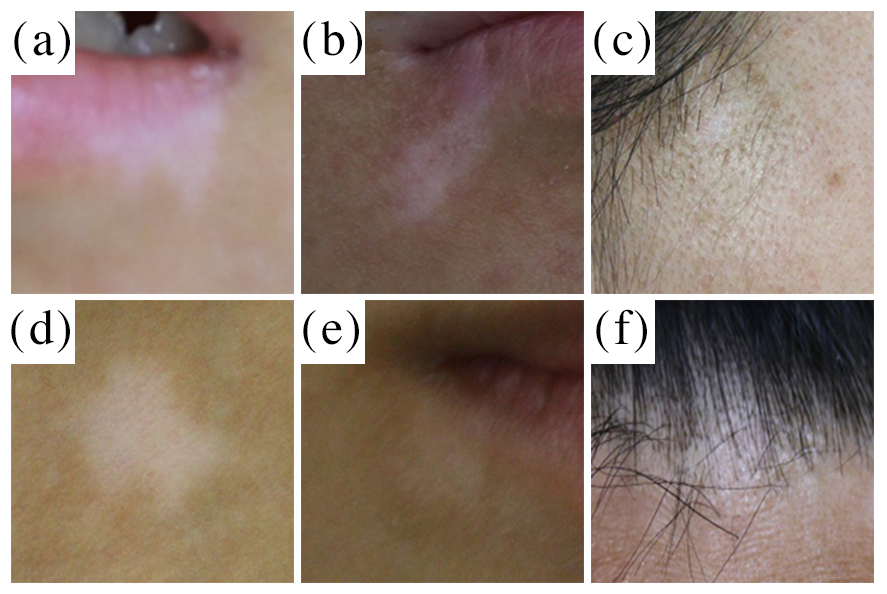
\includegraphics[width=0.7\linewidth]{chap1_challenge.jpg}
\end{center}
\caption{白癜风图像的例子和分割任务的挑战。}
\label{fig:chap1_challenge}
\end{figure}
如图\ref{fig:chap1_challenge},(a)-(d)展示了由于光照条件差和患者自身的肤色,皮损与健康皮肤之间的界限非常模糊。(e)对比度非常低。(c)和(f)都受到毛发的阻挡。由于(c)和(f)中的过渡曝光,部分健康皮肤容易被误认为是白癜风病变。

以上的各个因素,对于白癜风分割算法的要求非常高,如今应用于临床实践的算法很难满足需求。因此迫切需要抗干扰能力强,精度高且无需大规模精细标注的数据集支撑的分割算法。

\section{论文的研究工作}
本文首先对现有的白癜风评价体方法展开充分的研究,并进行了综合的对比。从而分析得出了以白癜风为代表的色素性皮肤病所具有的难点。然后指出分割问题是白癜风评价体系的核心问题。通过理论分析和实验验证指出了目前白癜风图像的分析和分割方法所区具有的缺陷,于是本文提出了一种基于显著性传播的弱监督分割方法。本文主要的工作有:

\begin{enumerate}
\item 综述了目前的白癜风评价指标,指出主观的评价体系的缺陷。从两个角度做了介绍,即色素性皮肤病分割与白癜风图像的分析与分割,并进行了细致的原理分析和优缺点对比。
\item 提出了到目前为止最大的一个白癜风数据集Vit2019,此数据集拥有1000张来自临床和网络的白癜风图片,并且均进行了白癜风区域的像素级标注。并从收集、标注、多样性与挑战四个方面介绍了该数据集。
\item 由于图像对比度低,皮损与正常皮肤过渡区域模糊等特点,提出了使用超像素分割方法作为图像预处理步骤,从而达到降低维度、剔除异常像素点、保留较完整准确的皮损边界等三个目的。
\item 由于图像大小尺寸不一致,引出了经典超像素分割算法中初始种子点数目确定难的问题,并针对提出了改进的方法。最后通过实验,定性的展示了超像素分割的效果,为下一章所介绍的弱监督分割框架奠定了基础。
\item 综述了目前先进的弱监督技术,并在此基础上,提出了面向白癜风等色素性皮肤病的分割框架。创新性的提出用于弱监督分割的“既见森林,又见树木”的策略,解释了如何将反馈的思想应用到显著性传播的过程中。最后通过多个实验验证了该方法的有效性,并与强监督学习的实验结果进行对比,发现在一些拍照环境恶劣,对比度很低的情况下,本文提出的方法甚至可以更好的分割白癜风区域并保持白癜风的边缘细节。
\end{enumerate}

\section{论文内容安排}
本论文正文共分为五个章节:

第一章是绪论,首先介绍了传统的白癜风评价指标,指出主观的评价体系的缺陷,以及提出一个客观评价体系的重要性和紧迫性。接着引出了客观评价体系的核心技术——分割。并对已有方法分别从两个角度做了介绍,即色素性皮肤病分割与白癜风图像的分析与分割,并进行了细致的原理分析和优缺点对比。通过分析目前方法所面临的挑战,引申出了本文的研究工作。

第二章是相关方法介绍。本章首先介绍了一些近些年来将深度学习应用于图像分割领域的方法和技术,然后着重介绍了一个经典的、具有代表性的网络结构——Unet。最后引出了基于强监督方法的缺点,即对数据集有很强的依赖性,为弱监督方法的引出进行了铺垫。然后本章对比了近年来各种弱监督分割方法,分析了其各自的优点和缺点,并将其基本的思想做了总结和归纳,为引出本文的弱监督分割框架进行了铺垫。最后,本章还介绍了一种简单而优雅的迭代聚类 算法——超像素分割 (SLIC),作为本文所提出的弱监督分割框架中的图像预处理步骤。将其应用于白癜风分割任务具有三个好处,即大大降低了维度、剔除一 些异常像素点、保留较完整准确的皮损边界。最后通过实验,定性的展示了超像素分割的效果,为之后所介绍的弱监督分割框架奠定了基础。


第三章是强监督分割。本章首先介绍了所提出的数据集 Vit2019,从收集、标注、多样性与挑战四个方面介绍了该数据集,并举例分析了部分样例图片。然后通过实验,定量和定性的展现并分析了Unet 在 Vit2019 上的效果,与之后的弱监督分割部分形成对照,用多项实验说明了本文所提出的弱监督分割方法可以很大程度的缩小与强监督方法效果之间的鸿沟。

第四章是弱监督分割框架,本章首先分析了在医疗图像处理领域对图像真值标注的困难性,然后提出了本文的方法,并详细介绍了每一步骤中的 原理以及意义。解释了如何做到 “既见森林,又见树木”,解释了如何将反馈的思想应用到显著性传播的过程中。然后说明了本框架应用于白癜风分割任务所带来的好处。最后通过多个实验验证了该方法的有效性,并与强监督学习进行对比,发现在一些拍照环境恶劣,对比度很低的情况下,本文提出的方法可以更好的分割白癜风区域并保持白癜风的边缘细节。

第五章是总结与展望。



















